\documentclass[a4paper,10pt]{article}
%\documentclass[a4paper,10pt]{scrartcl}

\usepackage{../mystyle}

\setromanfont[Mapping=tex-text]{Linux Libertine O}
% \setsansfont[Mapping=tex-text]{DejaVu Sans}
% \setmonofont[Mapping=tex-text]{DejaVu Sans Mono}
\parindent 0pt

\title{\sc Einführung in die Komplexe Analysis \\ \Large Blatt 1}
\author{Jendrik Stelzner}
\date{\today}

\begin{document}
\maketitle





\section{(Real und Imaginärteil)}
Es ist
\[
 \frac{i+1}{i-1} = \frac{i+1}{i(1+i)} = \frac{1}{i} = -i,
\]
und
\[
 \frac{3+4i}{2-i} = \frac{(3+4i)(2+i)}{(2-i)(2+i)} = \frac{2+11i}{5} = \frac{2}{5} + \frac{11}{5}i.
\]
Da $i^2 = -1$ (also insbesondere $i^4 = 1$) ist für alle $n \in \Z$
\[
 i^n =
 i^{(n \bmod 4)}
 \begin{cases}
   1 & \text{ falls } n \equiv 0 \mod 4, \\
   i & \text{ falls } n \equiv 1 \mod 4, \\
  -1 & \text{ falls } n \equiv 2 \mod 4, \\
  -i & \text{ falls } n \equiv 3 \mod 4.
 \end{cases}
\]
Schließlich ist
\[
 \left(\frac{1-i\sqrt{5}}{3}\right)^n
 = \Re \left(\frac{1-i\sqrt{5}}{3}\right)^n + i \Im \left(\frac{1-i\sqrt{5}}{3}\right)^n
\]
und
\begin{align*}
 \sum_{k=1}^7 \left(\frac{1+i}{\sqrt{2}}\right)^k
 &= \sum_{k=1}^7 e^{ik\pi/4}
 = \sum_{k=1}^3 e^{ik\pi/4} + \sum_{k=4}^7 e^{ik\pi/4} \\
 &= \sum_{k=1}^3 e^{ik\pi/4} + \sum_{k=0}^3 e^{ik\pi/4+i\pi} \\
 &= -1 + \sum_{k=1}^3 e^{ik\pi/4} + \sum_{k=1}^3 -e^{ik\pi/4} \\
 &= -1.
\end{align*}
Die entsprechenden Real- und Imaginärteile ergeben sich durch direktes Ablesen.





\section{(Betrag und Argument)}
Es ist
\[
 |1+3i| = \sqrt{1+3^2} = \sqrt{10} \text{ und } \arg (1+3i) = \arctan 3.
\]
Wegen der $2\pi$-Periodizität der Funktion $\R \to \C, t \mapsto e^{it}$ ist
\begin{align*}
 z_1
 &= (1+i)^9 - (1-i)^9
 = \left(\sqrt{2}e^{i\pi/4}\right)^9 - \left(\sqrt{2}e^{-i\pi/4}\right)^9 \\
 &= 2^{9/2} (e^{i\pi/4}-e^{i\pi/4})
 = 16 ((1+i)-(1-i)) \\
 &= 32i,
\end{align*}
also
\[
 |z_1| = 32 \text{ und } \arg z_1 = \frac{\pi}{2}.
\]
Da $i^2 = -1$ und $i^4 = 1$ ist $ z_2 = i^{2014} = -1$, also
\[
 |z_2| = 1 \text{ und } \arg z_2 = \pi.
\]
Für $z_3 = \frac{1+ia}{1-ia}$ ist
\[
 \left|z_3\right|
 = \frac{|1+ia|}{|1-ia|}
 = \frac{|1+ia|}{\left|\overline{1+ia}\right|}
 = 1,
\]
und da
\[
 \arg (1+ia) = \arctan a \text{ und } \arg (1-ia) = \arctan -a = - \arctan a.
\]
ist
\[
 \arg z_3 = \arg (1+ia) - \arg (1-ia) = 2 \arctan a.
\]
Für alle $n \in \Z$ und
\[
 z_n = (i-1)^n = \left(\sqrt{2}e^{i3\pi/4}\right)^n = \sqrt{2}^n e^{in3\pi/4}
\]
ist $|z_n| = \sqrt{2}^n$ und $n\frac{3}{4}\pi$ ein Argument von $z_n$.





\section{(Bestimmte Teilmengen)}


\subsection{}
Da $\Im(z) = 0 \Leftrightarrow z \in \R$ für alle $z \in \C$ und für alle $t \in \R, z \in \C$
\[
 \frac{z-3}{1+i} = t \Leftrightarrow z = 3+t(1+i)
\]
ist
\begin{align*}
 A_0
 &= \left\{ z \in \C : \Im\left( \frac{z-3}{1+i} \right) = 0 \right\}
 = \left\{ z \in \C : \frac{z-3}{1+i} \in \R \right\} \\
 &= \{ 3+t(1+i) : t \in \R \}.
\end{align*}
Es handelt sich bei $A_0$ also um eine Gerade.

Analog ergibt sich nun auch, dass
\begin{align*}
 A_+
 &= \left\{z \in \C : \Im\left( \frac{z-3}{1+i} \right) > 0 \right\} \\
 &= \left\{3 + t(1+i) + y(i-1) : t \in \R, y \in \R^+\right\}
\end{align*}
und
\begin{align*}
 A_-
 &= \left\{z \in \C : \Im\left( \frac{z-3}{1+i} \right) > 0 \right\} \\
 &= \left\{3 + t(1+i) + y(i-1) : t \in \R, y \in \R^-\right\}.
\end{align*}
Es ist also $A_+$ der Teil der komplexen Ebene, der über $A_0$ liegt, und $A_-$ der Teil der komplexen Ebene, der unter $A_0$ liegt.
Zusammengefasst ergibt sich die folgende Skizze.

\begin{center}
 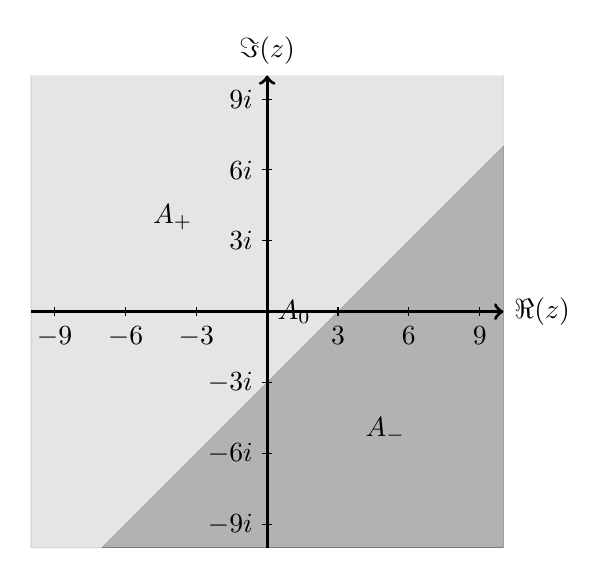
\begin{tikzpicture}[scale=0.3,domain=-7:10]
  \draw[very thick,->] (-10,0) -- (10,0) node[anchor=west] {$\Re(z)$}; % Re-Achse
  \draw[very thick,->] (0,-10) -- (0,10) node[anchor=south] {$\Im(z)$}; % Im-Achse
  % Beschriftung der Re-Achse
  \foreach \x in {-9,-6,-3,3,6,9}
   \draw (\x,1/5) -- (\x,-1/5) node[anchor=north] {$\x$};
  % Beschriftung der Im-Achse
  \foreach \y in {-9,-6,-3,3,6,9}
   \draw (1/5,\y) -- (-1/5,\y) node[anchor=east] {$\y i$};
  % Plote A_0
  \draw[thick] plot function {-3+x} node[anchor=west] {$A_0$};
  % Zeichne A_+ ein
  \draw[fill=black,opacity=0.1] (-10,10) -- (-10,-10) -- (-7,-10) -- (10,7) -- (10,10);
  \draw (-4,4) node {$A_+$};
  % Zeichne A_- ein
  \draw[fill=black,opacity=0.3] (-7,-10) -- (10,-10) -- (10,7);
  \draw (5,-5) node {$A_-$};
 \end{tikzpicture}
\end{center}





\subsection{}
Es ist $B = \emptyset$, denn für alle $z \in B$ ist
\[
 i = 3z\bar{z}+iz-i\bar{z}+2 = 3|z|^2 -2\Im(z) +2 \in \R.
\]





\section{(Kleine Stereograpische Projektion)}
Wir bemerken zunächst, dass der Ausdruck $(i\lambda+1)/(i\lambda-1)$ für alle $\lambda \in \R$ wohldefiniert ist, da stets $i\lambda-1 \neq 0$. Für alle $\lambda \in \R$ ist auch $i\lambda+1 \neq i\lambda-1$ (da $1 \neq -1$) und daher $(i\lambda+1)/(i\lambda-1) \neq 1$. Schließlich ist für alle $\lambda \in \R$
\[
 \left| \frac{i\lambda+1}{i\lambda-1} \right|
 = \frac{|i\lambda+1|}{|i\lambda-1|}
 = \frac{\sqrt{\lambda^2+1}}{\sqrt{\lambda^2+1}}
 = 1.
\]
Die Abbildung
\[
 \psi : \R \to S^1 \setminus \{1\}, \lambda \mapsto \frac{i\lambda+1}{i\lambda-1}
\]
ist also wohldefiniert.

Da jedes $z \in S^1 \setminus \{1\}$ eine eindeutige Darstellung als $z = e^{i\varphi}$ mit $\varphi \in (0,2\pi)$ hat, genügt es zum Nachweis der Bijektivität von $\psi$ zu zeigen, dass es für alle $\varphi \in (0,2\pi)$ genau ein $\lambda \in \R$ mit $\arg \psi(z) = \varphi$ gibt. (Wir fassen $\arg$ hier als eine Abbildung $\arg : \C \setminus \{0\} \to [0,2\pi)$ auf.)

Hierfür bemerken wir, dass für alle $\lambda \in \R$
\[
 \arg (i \lambda + 1) = \arctan \lambda
\]
sowie
\[
 \arg (i \lambda - 1) = \arg(-i \lambda + 1) - \pi = 2 \pi - \arctan (\lambda) - \pi = \pi - \arctan \lambda.
\]
Es ist also für alle $\lambda \in \R$
\[
 \arg \frac{i\lambda+1}{i\lambda-1}
 = 2\pi - \left( \arctan \lambda - (\pi - \arctan \lambda) \right)
 = \pi - 2\arctan \lambda.
\]
Da $\arctan : \R \to (-\pi/2,\pi/2)$ bijektiv ist zeigt dies nach der obigen Überlegung die Bijektivität von $\psi$.



















\end{document}
